\documentclass[10pt, journal]{IEEEtran}			% draftcls, http://vesta.informatik.rwth-aachen.de/ftp/pub/mirror/ctan/macros/latex/contrib/IEEEtran/IEEEtran_HOWTO.pdf
\usepackage{amsmath, amsthm, amssymb}
\usepackage{mathtools}
\usepackage[ngerman]{babel}	                    % Worttrennung nach deutschen standarts
\usepackage[utf8]{inputenc}                     % umlaute
\usepackage{geometry}			                % Randabstände einstellen
\usepackage[T1]{fontenc}	                    % deutsche Schriftzeichen
\usepackage{setspace}
\usepackage{graphicx}
\usepackage{parskip}
\usepackage{xcolor}
\usepackage{here}                               % Bilder hier her zwingen
\usepackage{subfig}                             % Bilder nebeneinander
\usepackage{siunitx}				            % Si Einheiten
\usepackage{gensymb}                            % ° in math
\usepackage{multirow}  				            % Multirow in Tabellen
\usepackage{arydshln}  				            % Punkt/strich Linen in Tabellen
\usepackage{lscape} 			            	% Seite kann mit landscape in Querformat dargestellt werden
\usepackage{tikz}                               % Kleine Koordinatensysteme
\usepackage{steinmetz}
\graphicspath{{./figures}}

\setlength\abovedisplayshortskip{-5pt}  		% Kopfabstand von Formeln
\setlength\abovedisplayskip{+7pt}
\setlength\belowdisplayskip{+7pt}
\geometry{left=2cm, top=1cm, bottom=1cm, right=1cm}
\definecolor{orange}{RGB}{255,120,0}
\definecolor{dgreen}{RGB}{0,95,0}
\definecolor{purple}{RGB}{200,0,255}
\usetikzlibrary{shapes.misc, angles, quotes, calc, patterns}    % Kreuz def., Winkel, Winkel
\tikzset{cross/.style=                          % Kreuz definition
    {cross out, draw=black, minimum size=2*(#1-\pgflinewidth), inner sep=0pt, outer sep=0pt},
    cross/.default={1pt}}                       % default radius = 1pt.
                                                % \RN für Römischezahl in math
\newcommand{\RN}[1]{\textup{\uppercase\expandafter{\romannumeral#1}}}
\newcommand{\ul}{\underline}
\renewcommand{\subitem}[1]{{\setlength\itemindent{15pt} \item[-] #1}}


\title{Formelsammlung EN}
\author{J/T/A}
\onehalfspacing

\begin{document}
\maketitle

\section{Grundlagen}
\subsection{Drehstrom (DS), 3-Phasen-System}
\begin{enumerate}


    \item{\textbf{Spannungen in DS (symmetrisch)}}\\
        \underline{Leiter-Erde-Spannung $U_{LE}=230V$}
        \begin{flalign*}
            \underline{U}_{L1} &= U_{LE} \angle 0^\circ &\\
            \underline{U}_{L2} &= U_{LE} \angle -120^\circ = U_{LE} \angle 240^\circ &\\
            \underline{U}_{L3} &= U_{LE} \angle -240^\circ = U_{LE} \angle 120^\circ &
        \end{flalign*}

        \underline{Leiter-Leiter-Spannung $U_{LL}=400V$}
        \begin{flalign*}
            U_{LL} &= U_{LE} \cdot \sqrt{3} &\\
            \underline{U}_{12} &= \underline{U}_{L1} - \underline{U}_{L2} = U_{LL} \angle 30^\circ &\\
            \underline{U}_{23} &= \underline{U}_{L2} - \underline{U}_{L3} = U_{LL} \angle 270^\circ &\\
            \underline{U}_{31} &= \underline{U}_{L3} - \underline{U}_{L1} = U_{LL} \angle 150^\circ &
        \end{flalign*}

    \item{\textbf{Ströme in DS (symmetrisch)}}
        \begin{flalign*}
            \underline{I}_{Lx} &= \dfrac{\underline{U}_{Lx}}{\underline{Z}} &
       \end{flalign*}

        $Lx:$ Stranggrößen L1, L2, L3\\

    \item{\textbf{Effektivgrößen, Symmetrische Last}}
        \begin{center}
            \vspace{-1em}
    \begin{tabular}[h]{l|l|l}
        Stranggröße & Stern & Dreieck
     \vspace{1pt}\\
        Spannung $U_{LE}$ & $U_{LE} = \dfrac{U_{LL}}{\sqrt{3}}$ & $U_{LE}=U_{LL}$\\
        Strom $I_L$ & $I_L = I_Z$ & $I_L = \sqrt{3}\cdot I_Z$
    \end{tabular}
    \vspace{0.5em}\\
    $I_Z:$ Strom in der Zuleitung, Betriebsstrom
    \end{center}

    \item{\textbf{Leistungen in DS}}

        \underline{Scheinleistung S [VA]:}
        \begin{flalign*}
        S &= 3 \cdot U_{LE} \cdot I_L
          = \sqrt{3} \cdot U_{LL} \cdot I_L &\\
          &= \sqrt{P^2 + Q^2} &\\
        \underline{S} &= 3 \cdot \underline{U}_{LE} \cdot \underline{I}_L^*
                      = P+jQ &
        \end{flalign*}
        \textit{in Sternschaltung:}
        \begin{flalign*}
        \underline{S}_{ds} &= \frac{U_{LL}^2}{\underline{Z}_{LN}*}  &\\
        \underline{S}_{ws}  &= \frac{U_{LL}^2}{3 \cdot \underline{Z}_{LN}*} &
        \end{flalign*}

        \underline{Wirkleistung P [W]:}
        \begin{flalign*}
        P   &= S \cdot \cos \varphi &\\
            &= 3 \cdot U_{LE} \cdot I_L \cdot \cos \varphi &\\
            &= \sqrt{3} \cdot U_{LL} \cdot I_L \cdot \cos \varphi &
        \end{flalign*}

        \underline{Blindleistung Q [var]:}
        \begin{flalign*}
        |Q| &= S \cdot \sin \varphi = P \cdot \tan \varphi &\\
            &= 3 \cdot U_{LE} \cdot I_L \cdot \sin \varphi &\\
            &= \sqrt{3} \cdot U_{LL} \cdot I_L \cdot \sin \varphi &\\
           & Q
            \begin{cases}
                \text{induktiv} >0\\
                \text{kapazitiv} <0
                \end{cases}
        \end{flalign*}
\end{enumerate}

\subsection{Energiebedarf, Deckung}
\begin{enumerate}
    \item{\textbf{Tagesbelastungskurve}}
\begin{flalign*}
    W &= \int_{0}^{T_{n}} P(t)  \,dt \\
      &= P_{n} \cdot T_{a} = P_{max} \cdot T_{m} =
    P_{mittel} \cdot T_{n}
\end{flalign*}

\begin{tabular}[h]{l|l}
    \hline
    $P_{n}$         & Nennleistung \\
    $T_{a}$         & Ausnutzungsdauer \\
    \hline
    $P_{max}$       & Höchstlast \\
    $T_{m}$         & Benutzungsdauer \\
    \hline
    $P_{mittel}$    & mittlere Leistung \\
    $T_{n}$         & Nennbetriebsdauer (meist. 24h) \\
\end{tabular}\\
\\
\item{\textbf{Frequenz-Wirkleistungs-Regelung}}
    		\item[a)]{\underline{stationärer Zustand (Gleichgewicht)}}
		\begin{align*}
			 W_{rot} = \frac{1}{2} \cdot J \cdot \omega_{mech} ^{2} &\qquad
			 \omega_{el} = p  \cdot \omega_{mech} \\
			%  \vspace{1pt}\\
			 W_{mech-zu} = W_{el-ab} &\qquad
			 P_{mech-zu} = P_{el-ab}
		\end{align*}

		$p$: Polpaarzahl \quad
		$J$: Massenträgheitsmoment\\

		\item[b)]{\underline{Störung}}
		% Sprunghafte Zunahme um $ \Delta P \Rightarrow$
		% Abbremsen der Rotoren $\Rightarrow$ Sinken der Drehzahl aller Generatoren
		% $\Rightarrow$ fehlende Energie wird aus gesp. Rotationsenergie aller elek.
		% Maschinen übernommen $\Delta W_{rot}$
		\begin{align*}
			W_{m-zu} \neq W_{el-ab} &\qquad
			P_{m-zu} \neq P_{el-ab} \\
			\Delta W_{rot} = \frac{1}{2} \cdot & J \cdot (\omega_{stat} - \omega_{akt})\\
		\end{align*}

\end{enumerate}

% \begin{gather*}
%     [R'] = [X'] = \frac{\Omega}{km} = \frac{m\Omega}{m} \\
%     [G'] = \frac{nS}{km} = \frac{pS}{m} \\
%     [B'] = \frac{\mu S}{km} = \frac{nS}{m}\\
%     B_{b}' = \omega C_{b}'
% \end{gather*}

\section{Trafo}
    OS:  Oberspannungsseite (Primär)\\
    US:  Unterspannungsseite (Sekundär)

    Index 1: $U_1:$ auf OS\\
    Index 2: $U'_2 = U_2 \cdot \ddot{u}:$ auf US
\vspace{-35pt}
\subsection{Grundgleichungen, idealer Trafo}
    % \item{\textbf{Windungsspannung}}
\begin{itemize}

    \item[]{\textbf{Windungsspannung}}
\begin{flalign*}
    \frac{U_{1}}{N_{1}} &= \frac{U_{2}}{N_{2}} = U_W = 4,44 \cdot f \cdot \hat{B} \cdot A_{Fe} &
\end{flalign*}

    \item[]{\textbf{Induktionsspannung, Effektivwert}}
    \begin{flalign*}
        U_{ieff} &= \frac{1}{\sqrt{2}} \cdot 2 \pi f \cdot N \cdot A_{Fe} \cdot
        \hat{B} &\\ &= 4,44 \cdot N \cdot f \cdot \hat{B} \cdot A_{Fe}
    \end{flalign*}

    \item[] \textbf{Transformation}\\


    \begin{tabular}[h]{c|c|c}
        \vspace{5pt}
        \textbf{Spannung} & \textbf{Strom} & \textbf{Impedanz} \\
        \vspace{5pt}
        $\dfrac{U_{1}}{U_{2}} = \dfrac{N_{1}}{N_{2}} = \ddot{u}$ & $\dfrac{I_{1}}{I_{2}} = \dfrac{N_{1}}{N_{2}} = \dfrac{1}{\ddot{u}}$ & $R'_{2} = \ddot{u}^2 \cdot R_{2}$\\
        \vspace{5pt}
        $\underline{U}'_{2}  = \ddot{u} \cdot \underline{U}_{2}$ & $\underline{I}'_{2} = \underline{I}_{2} \cdot \dfrac{1}{\ddot{u}}$ & $Z_1 = \ddot{u}^2 \cdot Z_2$\\
    \end{tabular}\\

    % \item[]{\textbf{Spannungstrafo}}
    % \begin{gather*}
    %     \frac{U_{1}}{U_{2}} = \frac{N_{1}}{N_{2}} = \ddot{u} \\
    %     \underline{U}'_{2}  = \ddot{u} \cdot \underline{U}_{2}
    % \end{gather*}
    % \item[]{\textbf{Stromtrafo}}
    % \begin{gather*}
    %     \frac{I_{1}}{I_{2}} = \frac{N_{1}}{N_{2}} = \frac{1}{\ddot{u}}\\
    %     \underline{I}'_{2} = \underline{I}_{2} \cdot \frac{1}{\ddot{u}}
    % \end{gather*}

    % \item[]{\textbf{Impedanztrafo}}
    % \begin{gather*}
    %     Z_{1} = \ddot{u}^2 \cdot Z_{2}\\
    %     R'_{2} = \ddot{u}^2 \cdot R_{2}\\
    %     L'_{2\sigma} = \ddot{u}^2 \cdot L_{2\sigma}
    % \end{gather*}

    \item[]{\textbf{Durchgangsleistung}}
    \begin{equation*}
        S_{1} = S_{2} = S_{D}
    \end{equation*}

\item[] {\textbf{Bemessungsscheinleistung [VA]}}
    \begin{align*}
        S_{rT} &= \sqrt{3} \cdot U_{LL,OS} \cdot I_{L,OS}\\
        S_{rT} &= 3 \cdot U_{LE,OS} \cdot I_{L,OS}
        \end{align*}

% \end{itemize}
% \textcolor{dgreen}{$R_{T}$ wird meist vernachlässigt}
% \vspace{-2em}
\subsection{Ersatzschaltbild (ESB)}
% \vspace{-2em}

\begin{gather*}
    U_1 = U_{OS} \qquad U'_2 = U_{US}\\
    R_{T} + jX_{T} = (R_1+R_2')+j(X_{1\sigma}+X'_{2\sigma})\\
    Z_{T} = R_{T} + jX_{T}\\
    U_1 = (R_T + jX_T) \cdot I_1 + U'_2
\end{gather*}

% \subsubsection{Leerlaufmessung}
% $\rightarrow R_{Fe}, X_{h}, P_{0T}$ \\\textcolor{dgreen}{Primärseitig $U_{rT1}$}\\
% % \textbf{Eisenwiderstand}\\
% % \textbf{Hauptreaktanz}\\
% % \textbf{Übersetzungsverhältnis}\\
% % \textbf{relativer Leerlaufstrom} \textcolor{dgreen}{(0.2 - 2\%)}
% \begin{gather*}
%     R_{Fe} \approx \frac{U_{rT1}/ \sqrt{3}}{I_{1}} \cdot \cos \phi = \frac{U_{rT1}^2}{P_{0T}}\\
%     X_{1h} \approx \frac{U_{rT1}/ \sqrt{3}}{I_{1}} \cdot \sin \phi = \frac{1}{i_{O}/100 \%} \cdot \frac{U_{rT1}^2}{S_{rT}}\\
%     \textnormal{"u} \approx \frac{U_{rT1}}{\sqrt{3} \cdot U_{2}}\\
%     i_{O} = \frac{I_{0}}{I_{rT}} \cdot 100\%
% \end{gather*}
\item[] {\textbf{Kurzschlussmessung (KS)}}

\setlength\parindent{20pt}\indent KS auf US. $\rightarrow  \underline{U}_{K1}$ auf OS (meistens)\\
\indent KS auf OS. $\rightarrow \underline{U}_{K2}$ auf US\\
% \begin{align*}
%     I_{K1} &= \frac{U_{1,LE}}{Z_{T1}} \qquad I_{K2} = \frac{U_{2,LE}}{Z_{T2}}\\
% \end{align*}

% \begin{itemize}
    \item[]{\textbf{Bemessungsspannung} (r = rated)}
    \[
    U_{rT} = U_{LL} = U_{LE} \cdot \sqrt{3}
    \]

    \item[]{\textbf{relative KS-Spannung [\%]}}
    \begin{align*}
        u_K  &= \sqrt{u^2_{K,Re}+u^2_{K,Im}}
             = \frac{U_K\cdot \sqrt{3}}{U_{rT}}\cdot 100\%\\
             &= \frac{Z_T \cdot I_r}{U_{rT}/\sqrt{3}}\\
    \ul{u}_{K1}  &= \frac{\ul{U}_{K1}}{ U_{rT1}/\sqrt{3} } =\frac{\ul{U}_{K1}}{U_{LE,T1}}\\
    \ul{u}_{K2} &= \frac{\ul{U}_{K2}}{ U_{rT2}/\sqrt{3}} = \frac{\ul{U}_{K1} \cdot \textnormal{ü}}{ U_{rT1} \cdot \textnormal{ü}/\sqrt{3}}\\
    u_{K,Re}      &= \frac{P_{K}}{S_{rT}}\cdot 100\%=\frac{R_T \cdot I_r}{U_{rT}/\sqrt{3}}\\
    u_{K,Im}  &= \sqrt{u^2_{K}-u^2_{K,Re}}
    \end{align*}

    \item[]{\textbf{KS-Größen}}
    \begin{align*}
    I_K &= \frac{I_r}{u_K} = \frac{U_{rT}/\sqrt{3}}{Z_T}\\
    U_K &= \frac{u_K}{100\%} \cdot \frac{U_{rT}}{\sqrt{3}}
    \end{align*}

    \item[]{\textbf{Betriebskonstanten}}
    \begin{align*}
    Z_T &= \frac{u_K}{100\%} \cdot \frac{U^2_{rT1}}{S_{rT}} \\
    R_T &= \frac{u_{K,Re}}{100\%} \cdot \frac{U^2_{rT1}}{S_{rT}} =
         \frac{u_{K,Re}}{100\%} \cdot \frac{U_{rT1}}{\sqrt{3}\cdot I_r}\\
        &= P_K \cdot \frac{U^2_{rT1}}{S^2_{rT}} = \frac{P_K}{3\cdot I^2_r}\\
    X_T &= \sqrt{Z^2_T - R^2_T} \quad \left(= u_{K,Im} \cdot \frac{U^2_{rT}}{S_{rT}} \right)
    \end{align*}

    \item[]{\textbf{Verlustleistung, Wirkungsgrad}}
\begin{align*}
    P_{ab} &= S_{rT} \cdot \cos \varphi\\
    P_{K,OS} &= 3 \cdot R_T \cdot I^2_{r,US}\\
    \eta &= \frac{P_{ab}}{P_{zu}} = \frac{P_{ab}}{P_{ab}+P_K+P_L}\\
    \eta_{max} &= \frac{P'_{ab}}{P'_{zu}} = \frac{S_{rT}\cdot \cos \varphi \sqrt{\frac{P_L}{P_K}}}{P'_{ab} + 2 P_L} \leftarrow P_L = P_K
    % I_{L,US} &= \sqrt{\frac{P_L}{3 \cdot R_T}} \leftarrow P_L = P_K
\end{align*}
$P_{ab}$: abgegebene Wirkleistung\\
$P_{K,OS}$: KS-/Kupferverluste, Index: $OS/US$\\
$I_r$: Bemessungsstrom auf $US$, wenn $P_K$ auf $OS$ \\
$P_L$: Leerlaufverluste\\
$\eta_{max}$: bei $P_L = P_K$


\subsection{Parallelbetrieb von 2 Trafos}
\item[] \textbf{Scheinleistungsteiler}
\begin{align*}
    |S_{T1}| &= \dfrac{Z_{T2}}{Z_{T1} + Z_{T2}} \cdot |S_{Tges}|\\
    |S_{T2}| &= \dfrac{Z_{T1}}{Z_{T1} + Z_{T2}} \cdot |S_{Tges}|\\
    |S_{Tges}| &= |S_{T1}| + |S_{T2}|\\
\end{align*}

\item[]{\textbf{max. Last, ohne Trafobelastung}}
    \begin{gather*}
    \left(\dfrac{S_{rT1/2}}{S_{T1/2}}\right)_{min} \Rightarrow S_{T,max} = \left(\dfrac{S_{rT}}{S_T}\right)_{min} \cdot S_{T,ges}\\
    S_{T1} = \dfrac{u_{K,min}}{U_{K,T1}} \cdot S_{rT1}
    \end{gather*}
\end{itemize}

\begin{enumerate}
    \item Schaltgruppe mit gleicher Kennzahl
    \item Gleiches Übersetzungsverhältnis
    \item annähernd gleiche Kurzschlussspannung (max. diff. 10\%)
    \item Bemessungsscheinleistung kleiner als 3:1
\end{enumerate}

\section{Freileitung}
\subsection{Durchhang von Freileitungsseilen}
hängen hyperbolisch durch. (ab \SI{110}{k\volt}:)
\begin{equation*}
    h_{min} = \SI{6}{\metre} + \left(\frac{U_{\mathit{nLL}} - \SI{110}{k\volt}}{\SI{150}{k\volt}}\right)m
\end{equation*}
\subsection{Resistanzbelag}
\begin{itemize}
\item[]{\textbf{Gleichstromwiderstand}}

$A_{\mathit{eff}}:$ Wirksamer Querschnitt [$mm^2$]\\
$F_{\vartheta}:$ Widerstandserhöhung durch Erwärmung\\
$\vartheta_{max}:$ max. zul. Betriebstemp. des Leiterseils

\begin{gather*}
    R_{\textcolor{purple}{=}}' = \frac{R_{=}}{l} = \frac{\rho_{20 \degree}}{A_{\mathit{eff}}}\cdot\frac{1}{km}\\
    F_{\vartheta} = 1 + \alpha (\vartheta_{max} - 20\degree C) + \beta (\vartheta_{max} - 20\degree C)...
\end{gather*}

\begin{table}[h]
\centering
\begin{tabular}[h]{|l|c|c|}
    \hline
    Material & $\rho_{\SI{20}{\degreeCelsius}}$ in $\frac{m\ohm \cdot mm^2}{m}$ & $\alpha$ in $K^{-1}$ \\
    \hline
    Alu & 28,6 & 0,0038 \\
    \hline
    Kupfer & 17,8 & 0,0039 \\
    \hline
    Silber & 16 & 0,0038 \\
    \hline
    Eisendraht & 120 & 0,0052 \\
    \hline
\end{tabular}
\end{table}

\item[]{\textbf{Wechselstromwiderstand}}
% \textbf{Stromdichte (Skineffekt)}\\
% \textbf{Eindringtiefe}\\
% \textbf{Gesamt Betriebswiderstand}
\begin{gather*}
    J = J \cdot e^{-x/\delta}\\
    \delta = \sqrt{ \frac{\rho}{\pi \cdot \mu_{0} \cdot f}}
     = \sqrt{ \frac{1}{\pi \cdot \kappa \cdot \mu_{0} \cdot f}}
\end{gather*}
$J:$ Stromdichte (Leiterrand)\\
$x:$ Abstand vom Leiterrand (Oberfläche)\\
$\delta:$ Eindringtiefe (Skineffekt)\\

\item[]{\textbf{Betriebs-Resistanzbelag}}
\begin{gather*}
    R_{b}' = R_{=}' \cdot F_{\vartheta} \cdot F_{S} = \frac{R_{b\mathtt{Seil}}'}{n_{\mathtt{Seil}}}
\end{gather*}
$F_S:$ Widerstandserhöhung durch Skineffekt
\newpage

\subsection{Induktivität}
\textbf{Aüßere Ind. Einzelleiter} \textcolor{dgreen}{mag. Fluss}\\
\textbf{-||- Doppelleiter}\\
\textbf{Innere Ind. Einzelleiter} \textcolor{dgreen}{verketteter mag. Fluss}\\
\textbf{-||- Doppelleiter}
\begin{gather*}
    \Phi_{a1} = \frac{\mu I l}{2 \pi} \cdot \ln \left( \frac{D-r}{r}\right)\\
    L_{a} = \frac{2\Phi_{a1}}{I} = \frac{\mu l}{2 \pi} \cdot \ln \left( \frac{D}{r}\right)\\
    \Psi_{i1} = \Psi_{i2} = \frac{\mu I l}{8 \pi}\\
    L_{i} = \frac{2\Psi_{i1}}{I} = \frac{\mu l}{8 \pi}
\end{gather*}

\textbf{gesamt Induktivität}\\
\textcolor{dgreen}{$\mu = \mu_{0}, D \gg r$}
\begin{gather*}
    L_{ges} = L_{a} + L_{i} = \frac{\mu l}{2\pi} \left( \ln \left(\frac{D}{r}\right) + \frac{1}{4}\right)\\
    L' = \frac{L_{ges}}{l} = \frac{\mu }{2\pi} \left( \ln \left(\frac{D}{r}\right) + \frac{1}{4}\right)
\end{gather*}

\subsection{Reaktanzbelag}
Metallmantel keine Schirmung! Für $D$ nicht $\gg r$!

\textbf{1- oder 2-Phasig}
\begin{equation*}
    X_{b}' = \pi \left( 4 \ln \left( \frac{D}{r}\right) +1 \right) \cdot 10 ^{-2}   \left[\frac{\Omega}{km}\right]
\end{equation*}

\textbf{Einfach-Drehstromkabel}
\begin{gather*}
    X_{b}' = \frac{\pi}{2} \left( 4 \ln \left( \frac{D_{m}}{r}\right) +1 \right) \cdot 10 ^{-2}   \left[\frac{\Omega}{km}\right]\\
    D_{m} = \sqrt[3]{D_{12} \cdot D_{23} \cdot D_{31}}
\end{gather*}

\textbf{Bündelleiter}
\begin{gather*}
    X_{b}' = \frac{\pi}{2} \left( 4 \ln \left( \frac{D_{m}}{r_{B}}\right) + \frac{1}{n} \right) \cdot 10 ^{-2}   \left[\frac{\Omega}{km}\right]\\
    r_{B} = \sqrt[n]{n \cdot r \cdot r_{T}^{n-1}}\\
    r_{T} = \frac{a}{2 \sin \frac{180 \degree}{n}}
\end{gather*}
Werden Bezeichnet nach: n x 2r / a

\textbf{Doppel 3-Phasig Bündelleiter}
\begin{gather*}
    X_{b}' = \frac{\pi}{2} \left( 4 \ln \left( \frac{D_{m} \cdot D_{L1/L\RN{2}}}{r \cdot D_{L1/L\RN{1}}}\right) + 1 \right) \cdot 10 ^{-2}   \left[\frac{\Omega}{km}\right]\\
    D_{L1/L\RN{2}} = \sqrt[3]{D_{1\RN{2}} \cdot D_{2\RN{3}} \cdot D_{3\RN{1}}}\\
    D_{L1/L\RN{1}} = \sqrt[3]{D_{1\RN{1}} \cdot D_{2\RN{2}} \cdot D_{3\RN{3}}}
\end{gather*}
Bei Asymmetrie (Phase zur Mastmitte)
\begin{equation*}
    D_{L1/L\RN{2}} = \sqrt[6]{D_{1\RN{2}} \cdot D_{2\RN{3}} \cdot D_{3\RN{1}} \cdot D_{1\RN{3}} \cdot D_{2\RN{1}} \cdot D_{3\RN{2}}}
\end{equation*}
\end{itemize}
\clearpage

\section{Kabel}

\subsection{Resistanzbelag}
\vspace{-2em}
\begin{align*}
    F_\vartheta &= 1+\alpha \cdot(\vartheta_{max} - 20\degree C)\\
    R'_b &=R'_=\cdot F_\vartheta \cdot F_S \cdot F_P
\end{align*}
$F_S$: Skineffekt (F35) \\
$F_P:$ Proximity-Effekt (F37)

\subsection{Reaktanzbelag}
Metallmantel keine Schirmung! Für $D$ nicht $\gg r$!\\
\indent $r:$ Radius des (Innen-)Leiters, nicht vom Mantel!

\textbf{Wechselstromkabel}
\begin{equation*}
    X_{b}' = \pi \left( 4 \ln \left( \frac{D}{r} -1\right) +1 \right) \cdot 10 ^{-2}   \left[\frac{\Omega}{km}\right]
\end{equation*}

\textbf{Einfach-Drehstromkabel}
\begin{equation*}
    X_{b}' = \pi \left( 2 \ln \left( \frac{D_{m}}{r} -1\right) +\frac{1}{2} \right) \cdot 10 ^{-2}   \left[\frac{\Omega}{km}\right]
\end{equation*}

\textbf{Doppel-Drehstromkabel}
\begin{equation*}
    X_{b}' = \pi \left( 2 \ln \left( \frac{D_{m} \cdot D_{L1L\RN{2}}}{r \cdot D_{L1L\RN{1}}} -1\right) +\frac{1}{2} \right) \cdot 10 ^{-2}   \left[\frac{\Omega}{km}\right]
\end{equation*}

\subsection{Suzeptanzbelag}
Metallmantel/-folie schirmt E-Feld ab!\\
\indent $B'_b:$ gilt für $f=50Hz$\\
\indent $d:$ Schirm/Mantel-Durchmesser eines Leiters\\
\indent $R:$ Radius der Isolierung\\
\indent $D:$ Abstand zw. 2 Innenleiter (vom Mittelpunkt)

\textbf{Einleiter-/Dreimantel-/Radialfeldkabel}
\begin{align*}
    C'_b &= C'_{LE} = \frac{2\pi \cdot \varepsilon_0 \cdot \varepsilon_r}{ln \left( \frac{R}{r} \right)}\\
    B'_b &= \omega C'_b  = \frac{17,47 \cdot \varepsilon_r}{ln \left(\frac{R}{r} \right)} \dfrac{\mu S}{km}
\end{align*}

\textbf{Wechselstromkabel - 2 Innenleiter}
\begin{align*}
    C_{b}' &= 2 \cdot C_{LE} + C_{LL} = \frac{\pi \cdot \varepsilon_{0} \cdot \varepsilon_{r}}{\ln \left( \left(\frac{D}{r}\right) \cdot \frac{(d^2 - D^2)}{(d^2 + D^2)} \right)}\\
    B'_b  &= \omega C'_b = \frac{8,735 \cdot \varepsilon_{r}}{\ln \left( \left(\frac{D}{r}\right) \cdot \frac{(d^2 - D^2)}{(d^2 + D^2)} \right)} \dfrac{\mu S}{km}
\end{align*}

\textbf{Einfach-Drehstromkabel - 3 Innenleiter}
\begin{align*}
    C_{b}' &= C_{LE} + 3 \cdot C_{LL} = \frac{4 \pi \cdot \varepsilon_{0} \cdot \varepsilon_{r}}{\ln \left( \left(\frac{D}{r}\right)^2 \cdot \frac{(0,75d^2 - D^2)^3}{(0,75d^2)^3 - (D^2)^3} \right)}\\
    B'_b &= \omega C'_b = \frac{34,94 \cdot \varepsilon_{r}}{\ln \left( \left(\frac{D}{r}\right)^2 \cdot \frac{(0,75d^2 - D^2)^3}{(0,75d^2)^3 - (D^2)^3} \right)}
     \dfrac{\mu S}{km}
\end{align*}
\indent keine Kopplung zum Nachbarsystem $B'_{\mathit{EDL}} = B'_{\mathit{DDL}}$

\subsection{Konduktanzbelag}
% \textcolor{dgreen}{Restleitfähigkeit der Isolierstoffe}
Ursache: Restleitfähigkeit der Isolierwerkstoffe\\ \indent bzw. Polarisationsverluste

\textbf{Verlustfaktor}
\begin{align*}
    \tan \delta &= \dfrac{I_{R}}{I_{C}} = \dfrac{1}{\omega C R} = \frac{G}{B}\\
    G_{b}' &= B_{b}' \cdot \tan \delta = \omega C_{b}' \cdot \tan \delta
\end{align*}
\begin{center}
\begin{tikzpicture}
    \draw[->] (-0.2,0) -- (3,0)         node[right] {$\ul{U}$};
    \draw[->] (0,-0.2) -- (0,2)         node[right] {$j$};
    \draw[->, red] (0,0) -- (2,0)       node[above left] {$\ul{I}_{R}$};
    \draw[->, green] (2,0) -- (2,2)     node[above right] {$\ul{I}_{C}$};
    \draw[->, blue] (0,0) -- (2,2)      node[above] {$\ul{I}$};
    \draw[<->] (45:0.5) arc (45:90:0.5) node[above right] {$\delta$};
\end{tikzpicture}

\end{center}

\textbf{Dielektrische Verluste}
\begin{align*}
    P_{Diel} &= (\tan \delta \cdot \varepsilon_{r}) \cdot \omega \cdot C_{\mathit{Vakuum}} \cdot U^2 = G'_b\cdot U^2_{LE}
\end{align*}
\indent $\tan \delta \cdot \varepsilon_{r}$: Verlustfaktor, siehe Tabelle \textbf{F43}

% \textcolor{red}{Werkstoff abhängige Verlustziffer}

\subsection{Leistung}
geg: $I_{max} , l , X'_b, G'_b$ \qquad ges: $P_{max}$
\begin{align*}
    X_b &= X'_b \cdot l \qquad B_b = B'_b \cdot l \\
    Q &= 3 \cdot I^2_{max} \cdot X_b - 3 \cdot U^2_{LE} \cdot B_b\\
    P_{max} &= \sqrt{S^2-Q^2}
\end{align*}

% \clearpage
\section{Betrieb von Leitungen}
\subsection{Kenngrößen}

\begin{itemize}
    \item[] \textbf{Leitung mit Verlusten}
    \begin{align*}
        \ul{\gamma} &= \sqrt{(R'_b +jX'_b)\cdot(G'_b+jB'_b)}= \alpha \cdot j \beta \left[\frac{\degree}{km} \right]\\
        \ul{Z}_w &= \sqrt{\dfrac{R'_b + jX'_b}{G'_b + jB'_b}}= |Z_w| \cdot e^{j\delta}
    \end{align*}
    \indent Falls Formel von $\ul{Z}_w$ nicht über TR berechenbar $\rightarrow$\\
    Betrag: erst $\ul{Z}_w^2$, dann $\sqrt{|Z_w^2|}$ ermitteln \\
    Phase: $0.5 \cdot \arg(\ul{Z}_w^2)$ \\

    \indent $\gamma:$ Ausbreitungskonstante\\
    \indent $\alpha:$ Dämpfungskonstante\\
    \indent $\beta:$ Phasenkonstante $[\frac{rad}{km} = \frac{180\degree}{\pi} \cdot \frac{1}{km} = \frac{\degree}{km}]$\\
    \indent $Z_w:$ Wellenwiderstand\\
    \indent $\delta:$ Phase des Wellenwiderstandes\\

    \item[] \textbf{Leitung ohne Verluste}\\
            $R'_b = G'_b = 0\rightarrow \alpha, \delta = 0$
        \begin{align*}
            \ul{\gamma} &= j \beta = j \sqrt{X'_b \cdot B'_b} = j \omega \cdot \sqrt{L'_b \cdot C'_b}\left[\frac{\degree}{km} \right]\\
            |\beta| &= \sqrt{X'_b \cdot B'_b} \cdot \frac{180\degree}{\pi} = \omega \cdot \sqrt{L'_b \cdot C'_b} \\
            |Z_w| &= \sqrt{ \dfrac{X'_b}{B'_b} } = \sqrt{ \dfrac{L'_b}{C'_b} }
        \end{align*}
    Richtwerte:
            $Z_w \approx 400\: \ohm \qquad \beta = \frac{0,06\degree}{km}$\\

    \item[] \textbf{natürliche Leistung, Blindleistungsverluste}

        - gilt bei Leitung ohne Verlusten, DS-System\\
        - natürlicher Betrieb bei $Q_L = Q_C$
        \begin{align*}
            I_{nat} &= \frac{U_{LE}}{\sqrt{X_L/B_L}} =  \frac{U_{LE}}{Z_w} \neq f(l)\\
            P_{nat} &= 3 \cdot U_{LE} \cdot I_{nat} = \frac{U^2_{LL}}{Z_w} = \frac{3 \cdot U_{LE}}{Z_w}\\
            Q_L &= 3 \cdot X_L \cdot I_L^2 \qquad Q_C = 3 \cdot B_L \cdot U^2_{LE}\\
            \frac{Q_V}{Q_C} &= \left(\frac{S_u}{P_{nat}} \right)^2-1\\
            Q_v &= Q_1 - Q_2 = Q_L - Q_C = Q_C \cdot (\frac{Q_L}{Q_C}-1)\\
            S_v &= S_1 - S_2 = P_v + j Q_v\\
            S_u &= 3 \cdot U_{LE} \cdot I_L = \sqrt{3} \cdot U_{LL} \cdot I_L
        \end{align*}

        \indent $Q_v:$ Blindleistungsverluste\\
        \indent $S_u:$ Übertragungsscheinleistung

\subsection{Ersatzschaltbilder (ESB)}

\textbf{Kenngrößen}\\

\begin{tabular}[h]{c|c|c}
    & Längszweig & Querzweig $\parallel$ \\
    \hline
    Wirk & $R_L = R'_b \cdot l$ & $G_L= G'_b \cdot l$\\
    Blind & $X_L = X'_b \cdot l$ & $B_L = B'_b \cdot l$\\
    % Blind & $X_L = X'_b \cdot l$ & $B_L = B_'b \cdot l$\\
\end{tabular}\\

$R_L$: Resistanz \qquad $X_L$: Reaktanz\\
$B_L$: Suszeptanz \qquad $G_L$: Konduktanz\\

Index $1/\ul{2}$: Größe am Anfang/\ul{Ende} der Leitung\\
Index $L$: Größen bezogen auf Leitung\\
$dU$: Spannung am Längszweig\\

\newpage
\item[] \textbf{MS-/NS-Leitungen mit Verlusten}\\
    $I_G, I_C<< I_L \Rightarrow G'_b = B'_b = 0$
        \begin{align*}
            \ul{I_1} &= \ul{I}_L = \ul{I}_2 \qquad
            \ul{U}_1 = d \ul{U} + \ul{U}_2\\
            d \ul{U} &= (R_L + jX_L) \cdot \ul{I}_L = (R'_b +jX'_b) \cdot l \cdot \ul{I}_L\\
            \ul{Z}_L &= R_L +jX_L \qquad \varphi_Z =\arctan \frac{X_L}{R_L} = \arctan \frac{X'_b}{R'_b}
        \end{align*}

\item[] \textbf{\ul{Kurze} HS-/HöS-DS-Freileitungen}

    $U_{LL}$ > 100 kV für $l\leq$ 220 km\\

    \ul{ohne Verluste:} ($R'_b = G'_b = 0$)
    \begin{align*}
        B'_1 &= B'_2 = \frac{B'_b}{2} \qquad
        \ul{I}_{C1/2} = j \: B_{1/2} \cdot \ul{U}_{1/2}\\
        \ul{I}_1 &= \ul{I}_{C1} + \ul{I}_L \qquad  \ul{I}_L =  \ul{I}_{C2} +  \ul{I}_2
         % \ul{U}_1 = d\ul{U} + \ul{U}_2 = (R_L + jX_L) \cdot \ul{I}_L + \ul{U}_2\\
    \end{align*}
    \textit{bei Leerlauf:} $\ul{I}_2 = 0 \rightarrow \ul{I}_{C2} = \ul{I}_L$
    \begin{align*}
        \ul{U}_1 &= (1 - \frac{X_L\cdot B_L}{2}) \cdot \ul{U}_2\\
        \ul{I}_1 &=  \ul{I}_2 + j \: 0.5 \cdot B_L \cdot ( \ul{U}_1 + \ul{U}_2)\\
        Q_1 &= 3\cdot U_1 \cdot I_1
    \end{align*}
    $\ul{I}_1$: Ladestrom \qquad
    $Q_1:$ Ladeleistung\\

    \textit{bei Betrieb mit natürlicher Leistung}: $R_2 = Z_w = \ul{Z}_2$
        \begin{align*}
            S_1 = S_2 &= P_1 = P_2 = P_{nat} \quad
            |\ul{U}_1| = |\ul{U}_2| \quad |I_1| = |I_2|\\
            \ul{U}_1 &= \ul{U}_2 \cdot(1-\frac{1}{2} \cdot B_L \cdot X_L + j\: \frac{X_L}{Z_w})\\
            \ul{I}_1 &= \frac{\ul{U}_2}{Z_w}+j\: \frac{B_L}{2}\cdot (\ul{U}_1 + \ul{U}_2)\\
            \ul{I}_L &= \frac{\ul{U}_2}{Z_w}+j\: \frac{B_L}{2}\cdot \ul{U}_2\\
        \end{align*}

\item[] \textbf{\ul{Lange} HS-/HöS-DS-Freileitungen}

    $U_{LL}$ > 100 kV für $l>$ 220 km\\

    \ul{ohne Verluste} ($R'_b = G'_b = 0$)
    \begin{align*}
        \ul{U}_1 &= \ul{U}_2 \cdot \cos(\beta l) + j \cdot \ul{I}_2 \cdot Z_w \cdot \sin (\beta l)\\
        \ul{I}_1 &= \ul{I}_2 \cdot \cos(\beta l) + j \cdot \frac{\ul{U}_2}{Z_w} \cdot \sin (\beta l)
    \end{align*}
    \textit{bei Leerlauf:} $\ul{I}_2 = 0$, $\ul{Z}_2 \rightarrow \infty$\\
    \textit{bei Betrieb mit natürlicher Leistung:} $\varphi = \beta l$
    \begin{align*}
        \ul{U}_1 &= |\ul{U}_2| \cdot e^{j\varphi} \qquad
        \ul{I}_1 = |\ul{I}_2| \cdot e^{j\varphi}\\
        \ul{S}_1 &= \ul{S}_2 = \frac{3 \cdot U_{2,LE}^2}{Z_w} = P_{nat}
    \end{align*}

    \ul{mit Verlusten}
    \begin{align*}
        \ul{U}_1 &= \ul{U}_2 \cdot \cosh(\ul{\gamma} l) + \ul{I}_2 \cdot \ul{Z}_w \cdot \sinh(\ul{\gamma} l)\\
        \ul{I}_1 &= \ul{I}_2 \cdot \cosh(\ul{\gamma} l) + \frac{\ul{U}_2}{\ul{Z}_w}\cdot \sinh(\ul{\gamma} l)
    \end{align*}
    nicht direkt mit komplexen Modus des TR einsetzbar!\\
    Lösung: $\alpha \cdot l $ und $ \beta \cdot l [\degree]$ einzeln berechnen, dann:
    \begin{align*}
        \cosh(\ul{\gamma}l) &= \frac{1}{2} \left[e^{\alpha l} \cdot e^{j\beta l} + e^{-\alpha l} \cdot e^{-j\beta l} \right]\\
        \sinh (\ul{\gamma}l)&= \frac{1}{2} \left[e^{\alpha l} \cdot e^{j\beta l} - e^{-\alpha l} \cdot e^{-j\beta l} \right]\\
        % \ul{U}_1 = \ul{U}_2 \cdot  \frac{1}{2} \left[e^{\alpha l} \cdot e^{j\beta l} + e^{-\alpha l} \cdot e^{-j\beta l} \right]\\
        % + \ul{I}_2 \cdot \ul{Z}_w \cdot \frac{1}{2} \left[e^{\alpha l} \cdot e^{j\beta l} - e^{-\alpha l} \cdot e^{-j\beta l} \right]\\
        % \ul{I}_1 = \ul{I}_2 \cdot  \frac{1}{2} \left[e^{\alpha l} \cdot e^{j\beta l} + e^{-\alpha l} \cdot e^{-j\beta l} \right]\\
        % + \ul{I}_2 \cdot \ul{Z}_w \cdot \frac{1}{2} \left[e^{\alpha l} \cdot e^{j\beta l} - e^{-\alpha l} \cdot e^{-j\beta l} \right]\\
    \end{align*}

\item[] \textbf{HS-/HöS-DS-Kabel}

    $l>95km$: langes Kabel\\
    $Q_V = Q_L - Q_C$ wie Freileitungen (FL), aber $Q_K > Q_{FL}$
    \begin{align*}
        S_{th}&= 3\cdot U_{LE}\cdot I_{Dauer}\\
        P_{max}&= \sqrt{S^2_{th}-Q^2_V} = \sqrt{S^2_{th} - Q'^2_V \cdot l^2}\\
        Q_V &= Q'_V \cdot l \qquad l_{max}= \frac{S_{th}}{Q'_v}
    \end{align*}

    $S_{th}$: thermisch, max. Scheinleistung\\
    $P_{max}$: max. übertragbare Wirkleistung\\
    $l_{max}$: max. Kabellänge, wenn $P_{max} = 0$

\end{itemize}

\section{Generator}
\textbf{Induktionsgesetz}\\
\textbf{Polpaarzahl}
\begin{align*}
    U_{ieff} &= 4,44 \cdot N \cdot f \cdot B_= \cdot \hat{A}_{Fe} \\
    n &= \dfrac{3000}{p} \left[ \frac{1}{min}\right] \qquad \textnormal{für f = 50Hz}
\end{align*}

\subsection{Ersatzschaltbild (ESB)}
\begin{align*}
    \ul{U}_p &= \ul{U} + (R_S + jX_S) \cdot \ul{I} \qquad \textnormal{$R_S$ wird meist vernachl.}\\
    1 &= \left( \dfrac{U}{U_p} \right)^2 - 2 \cdot \left( \dfrac{U \cdot I}{U_p \cdot I_k}\right) sin(\varphi) + \left(\dfrac{I}{I_k}\right)^2
\end{align*}

\subsection{Alleinbetrieb (Inselbetrieb)}
\subsubsection{Reine Wirkleistung}
\begin{align*}
    cos(\varphi) &= 1\\
    1 &= \left( \dfrac{U}{U_p} \right)^2 + \left(\dfrac{I}{I_k}\right)^2
\end{align*}

\subsubsection{Reine Blindleistung}
\begin{align*}
    sin(\varphi) &= 1 \rightarrow (ind.) \qquad =-1 \rightarrow (kap.)\\
    \left( \dfrac{U}{U_p} \right) &= 1 \mp \left(\dfrac{I}{I_k}\right)
\end{align*}

\subsection{Leistung}
\begin{align*}
    S_{Bez} &= 3 \cdot \dfrac{U^2}{X_S}\\
    \dfrac{P}{S_{Bez}} &= \left(\dfrac{U_p}{U}\right) sin(\upsilon)\\
    P_{mech,zu} &= P_{el,ab} \neq f(\upsilon) \rightarrow \textnormal{für $\upsilon < 90\degree$ stabil}\\
    \dfrac{Q}{S_{Bez}} &= \left(\left(\dfrac{U_p}{U}\right) cos(\upsilon)\right) -1\\
    P_{Kipp} &= 3 \cdot \dfrac{U \cdot U_p}{X_S}
\end{align*}
\onecolumn
\section{Tabellen, Anhänge}
% \centering
\large
\textbf{F39 - Gleichstromwiderstand, Seildurchmesser, Sollquerschnitt (Freileitung)}

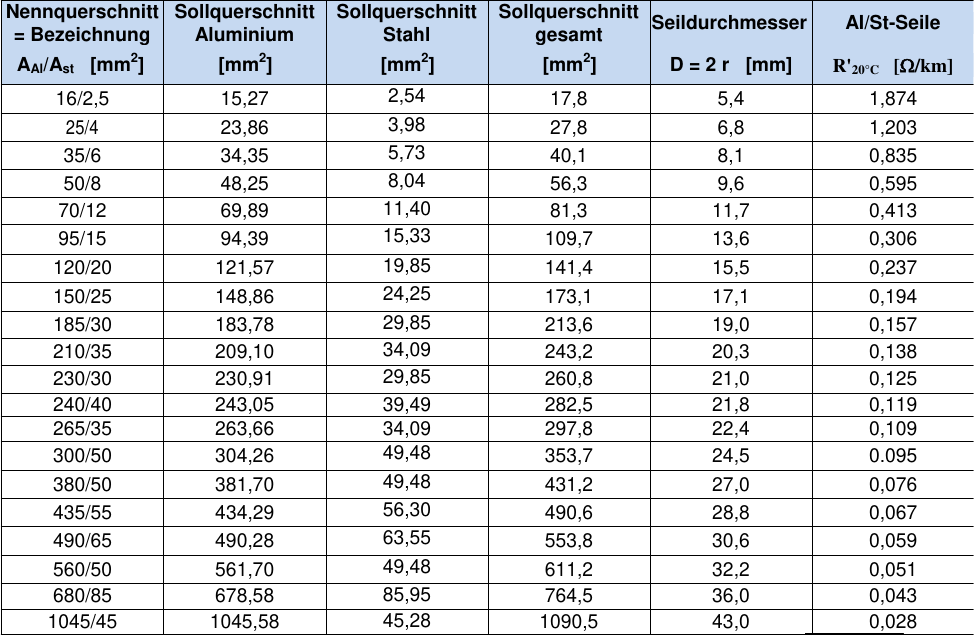
\includegraphics[width=0.9\columnwidth]{figures/freileitung_f39_resistanzbelag.png}

\textbf{F42 - Widerstandserhöhung durch Skineffekt (Freileitung, Kabel)}

\includegraphics[width=0.9 \columnwidth]{figures/f_42_widerstandserhöhung_skineffekt.png}

\newpage
\textbf{F43 - Resistanzbelag, Richtwerte Seilbelegungen (Freileitung)}

\begin{center}
\begin{tabular}[h]{|c|c|c|}
    \hline
    Leitung $[kV]$ & Seiltyp & $R'_b \left[ \frac{\Omega}{km} \right]$ \\
    \hline
    10/20 & Einfach& 0,3 - 0,6 \\
    \hline
    110 & Einfach& 0,2 - 0,15\\
    \hline
    220 & Zweierbündel& 0,09\\
    \hline
    380 & Viererbündel & 0,03\\
    \hline
\end{tabular}
\end{center}

\textbf{F46 - Reaktanzbelag, Richtwerte Hochspannungsleitungen (Freileitung)}

\makebox[\textwidth][c]
{
\begin{minipage}{0.5\textwidth}
\begin{tabular}{|c|c|}
    \hline
    Seiltyp & $X'_b \left[ \frac{\Omega}{km} \right]$ je Leiter \\
    \hline
    Einerseil & 0,40 \\
    \hline
    Zweierbündel & 0,30 \\
    \hline
    Viererbündel & 0,23 \\
    \hline
\end{tabular}
\end{minipage}
\hspace{-5em}
\begin{minipage}[c]{0.5\textwidth}
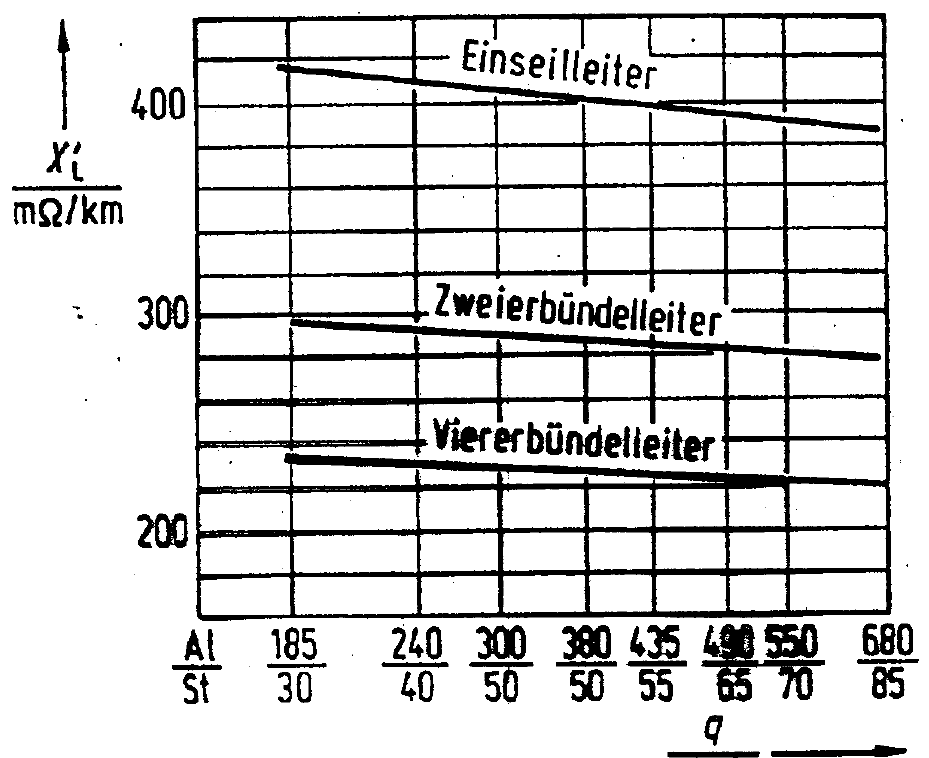
\includegraphics[width=\columnwidth]{figures/f46_freileitung_reaktanzbelag.png}
\end{minipage}
}

\textbf{F48 - Suszeptanzbelag, Richtwerte Einfachseil bei f=50Hz (Freileitung)}

\makebox[\textwidth][c]
{
\begin{minipage}{0.5\textwidth}
\begin{tabular}{|c|c|}
    \hline
    Richtwerte $U_{Betrieb}$ & $B'_b \left[ \frac{\mu S}{km} \right]$ je Leiter \\
    \hline
    < 30 kV & 3,5 \\
    \hline
    > 30 kV & 3 \\
    \hline
\end{tabular}
\end{minipage}
\hspace{-5em}
\begin{minipage}[c]{0.5\textwidth}
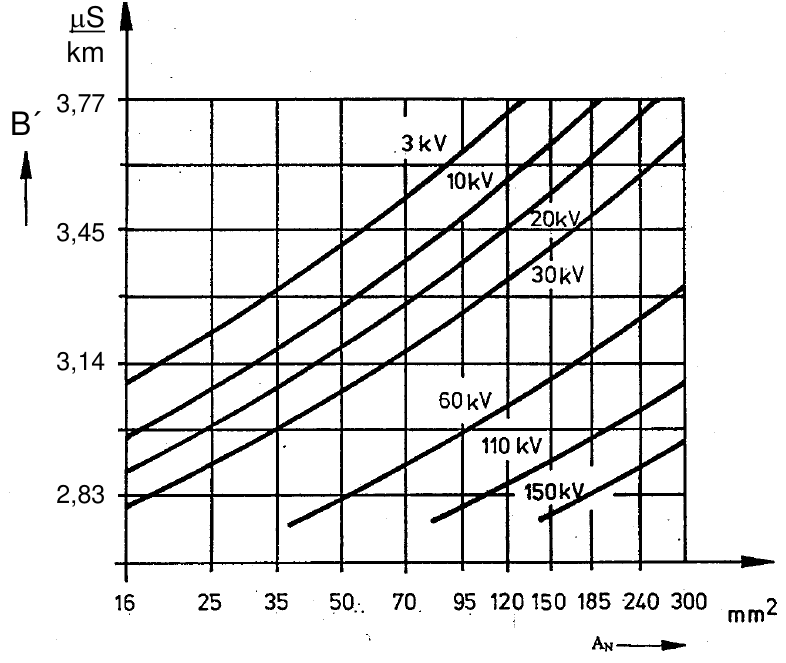
\includegraphics[width=\columnwidth]{figures/f_48_freileitung_suszeptanzbelag.png}
\end{minipage}
}

\textbf{F49 - Konduktanzbelag, Richtwerte (Freileitung)}

\makebox[\textwidth][c]
{
\begin{minipage}{0.5\textwidth}
\begin{tabular}{|c|c|}
    \hline
    Richtwerte $U_{Betrieb}$ & $G'_b \left[ \frac{nS}{km} \right]$ je Leiter \\
    \hline
    < 30 kV & vernachlässigbar \\
    \hline
    100 kV & 4 - 5 \\
    \hline
    220 kV & 2,5 - 3,5 \\
    \hline
    380 kV & 1 - 2\\
    \hline
\end{tabular}
\end{minipage}
\hspace{-5em}
\begin{minipage}{0.5\textwidth}
\begin{itemize}
    \item Strom über Isolation (hier Luft) gegen Erde
    \item Ursachen: Korona- und Isolationsverluste
\end{itemize}
\end{minipage}
}

\newpage


\textbf{F34 - Resistanzbelag $R'_{=}$ in $\frac{\Omega}{km}$ (Kabel)}

\makebox[\textwidth][c]
{
\begin{minipage}{0.5\textwidth}

\begin{tabular}{|c|c|}
    \hline
    Seiltyp & $X'_b \left[ \frac{\Omega}{km} \right]$ je Leiter \\
    \hline
    Einerseil & 0,40 \\
    \hline
    Zweierbündel & 0,30 \\
    \hline
    Viererbündel & 0,23 \\
    \hline
\end{tabular}
\end{minipage}
\hspace{-5em}
\begin{minipage}[c]{0.5\textwidth}
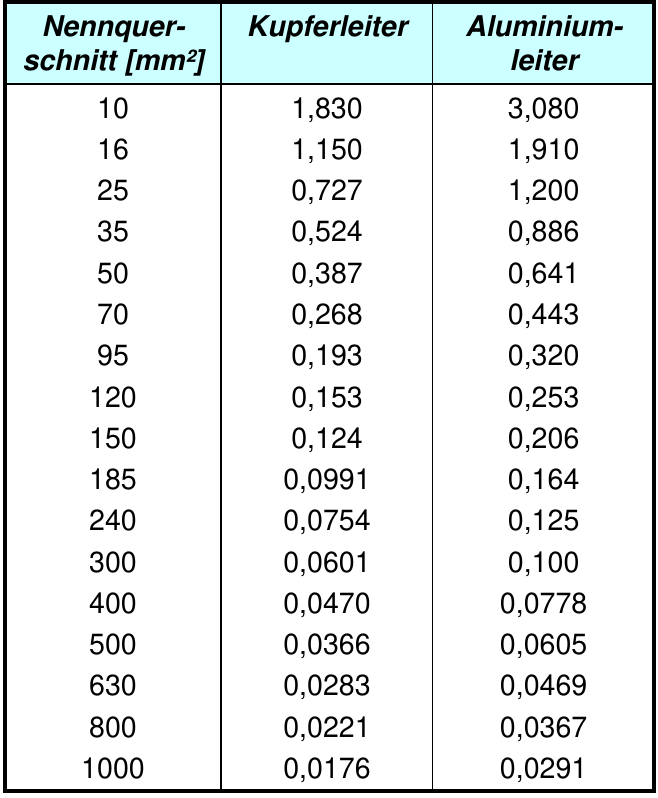
\includegraphics[width=0.8\columnwidth]{figures/f34_Kabel_Gleichstromwiderstand.png}
\end{minipage}
}

\textbf{F37 - Widerstandserhöhung durch Proximityeffekt (Kabel)}

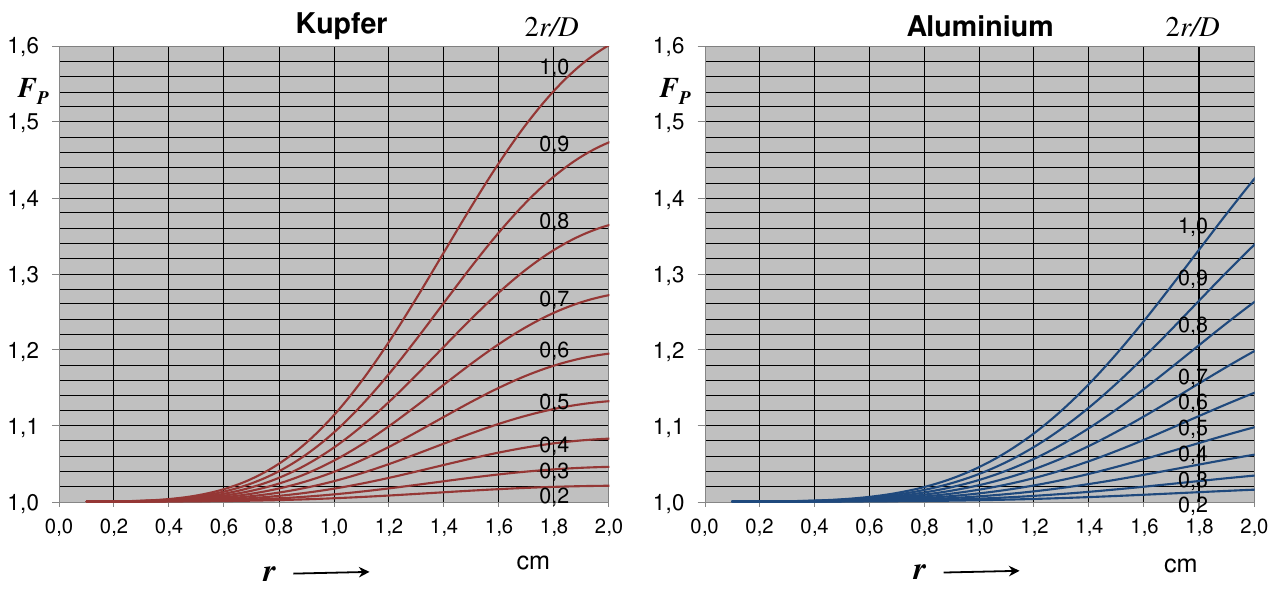
\includegraphics[width=0.96\columnwidth]{figures/F37_Kabel_Resistanzbelag_Proximityeffekt.png}


\end{document}
